%%%%%%%%%%%%%%%%%%%%%%%%%%%%%%%%%%%%%%%%%
% Jacobs Landscape Poster
% LaTeX Template
% Version 1.0 (29/03/13)
%
% Created by:
% Computational Physics and Biophysics Group, Jacobs University
% https://teamwork.jacobs-university.de:8443/confluence/display/CoPandBiG/LaTeX+Poster
% 
% Further modified by:
% Nathaniel Johnston (nathaniel@njohnston.ca)
%
% This template has been downloaded from:
% http://www.LaTeXTemplates.com
%
% License:
% CC BY-NC-SA 3.0 (http://creativecommons.org/licenses/by-nc-sa/3.0/)
%
%%%%%%%%%%%%%%%%%%%%%%%%%%%%%%%%%%%%%%%%%

%----------------------------------------------------------------------------------------
%	PACKAGES AND OTHER DOCUMENT CONFIGURATIONS
%----------------------------------------------------------------------------------------

\documentclass[final,table]{beamer}
\usepackage{xcolor}
\usepackage[scale=1.24]{beamerposter} % Use the beamerposter package for laying out the poster

\usetheme{confposter} % Use the confposter theme supplied with this template
\usepackage{graphicx}
\usepackage{caption}
\usepackage{wrapfig}
\usepackage{tikz}
\usepackage{subcaption}
\setbeamercolor{block title}{fg=ngreen,bg=white} % Colors of the block titles
\setbeamercolor{block body}{fg=black,bg=white} % Colors of the body of blocks
\setbeamercolor{block alerted title}{fg=white,bg=dblue!70} % Colors of the highlighted block titles
\setbeamercolor{block alerted body}{fg=black,bg=dblue!10} % Colors of the body of highlighted blocks
% Many more colors are available for use in beamerthemeconfposter.sty

%-----------------------------------------------------------
% Define the column widths and overall poster size
% To set effective sepwid, onecolwid and twocolwid values, first choose how many columns you want and how much separation you want between columns
% In this template, the separation width chosen is 0.024 of the paper width and a 4-column layout
% onecolwid should therefore be (1-(# of columns+1)*sepwid)/# of columns e.g. (1-(4+1)*0.024)/4 = 0.22
% Set twocolwid to be (2*onecolwid)+sepwid = 0.464
% Set threecolwid to be (3*onecolwid)+2*sepwid = 0.708

\newlength{\sepwid}
\newlength{\onecolwid}
\newlength{\twocolwid}
\newlength{\threecolwid}
\setlength{\paperwidth}{48in} % A0 width: 46.8in
\setlength{\paperheight}{36in} % A0 height: 33.1in
\setlength{\sepwid}{0.024\paperwidth} % Separation width (white space) between columns
\setlength{\onecolwid}{0.22\paperwidth} % Width of one column
\setlength{\twocolwid}{0.464\paperwidth} % Width of two columns
\setlength{\threecolwid}{0.708\paperwidth} % Width of three columns
\setlength{\topmargin}{-0.5in} % Reduce the top margin size
%-----------------------------------------------------------

\usepackage{graphicx}  % Required for including images

\usepackage{booktabs} % Top and bottom rules for tables
\definecolor{color1}{HTML}{FF66CC}
\definecolor{color2}{HTML}{4D90FE}
\definecolor{green}{HTML}{99FF99}
\definecolor{red}{HTML}{FF9999}
\definecolor{yellow}{HTML}{FFFF99}
\newcommand{\spar}{\vspace{26pt}\noindent}

%----------------------------------------------------------------------------------------
%	TITLE SECTION 
%----------------------------------------------------------------------------------------

\title{ \
Get Rich - \underline{G}eneralized \underline{E}xamination of \underline{T}weets for\\ \underline{R}ecommendations of \underline{I}nvestment and Sto\underline{c}k Purc\underline{h}asing   \hspace{1ex} 
          }
          
\author{Jonathan Sumrall, Sander Kools, Giedo Mak, and Michiel Fortuin } % Author(s)

\institute{Technical University of Eindhoven} % Institution(s)

%----------------------------------------------------------------------------------------

\begin{document}
\addtobeamertemplate{block end}{}{\vspace*{2ex}} % White space under blocks
\addtobeamertemplate{block alerted end}{}{\vspace*{2ex}} % White space under highlighted (alert) blocks

\setlength{\belowcaptionskip}{2ex} % White space under figures
\setlength\belowdisplayshortskip{2ex} % White space under equations

\begin{frame}[t] % The whole poster is enclosed in one beamer frame

\begin{columns}[t] % The whole poster consists of three major columns, the second of which is split into two columns twice - the [t] option aligns each column's content to the top

\begin{tikzpicture}[overlay, remember picture]
\path (current page.north east) ++(-2,-2) node[below left] {
\includegraphics[width=25ex]{logo.png}};
\end{tikzpicture}
\begin{tikzpicture}[overlay, remember picture]
\path (current page.north west) ++(13,-1) node[below left] {
\includegraphics[width=20ex]{getrichlogo.png}};
\end{tikzpicture}


\begin{column}{\twocolwid} % The first column

\begin{block}{Goal}
\centering
\emph{Using a general sample of tweets, calculate  daily mood trends and predict future prices of key stock market indexes. }
\newline
\end{block}

\begin{block}{Data}
We collected tweets from Twitter, who provide a stream of tweets as they arrive. Historical tweets from Archive.org were used for testing and development. 

\begin{figure}
          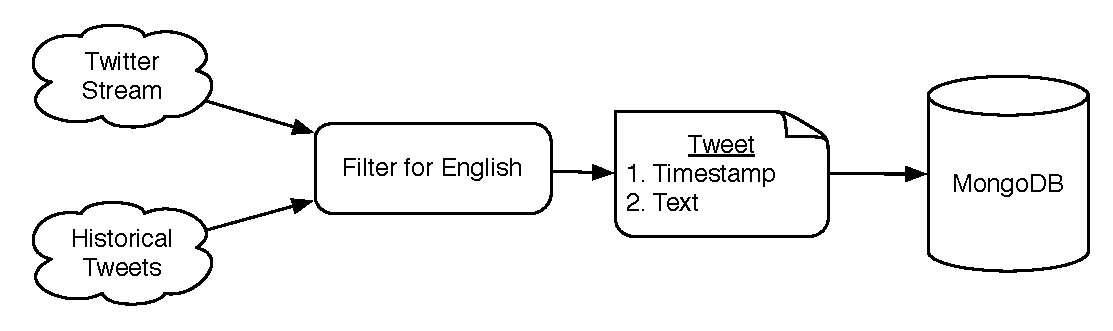
\includegraphics[width=70ex]{tweet_filtering.pdf}
          \caption{Data collection process}
\end{figure}


\end{block}


\begin{block}{Sentiment analysis}
Sentiment analysis is perform on each tweet. We determine the mood based on Plutchik's wheel of emotions. 

%\begin{wrapfigure}{R}{0.6\textwidth}
\begin{center}
\begin{figure}[ht!]
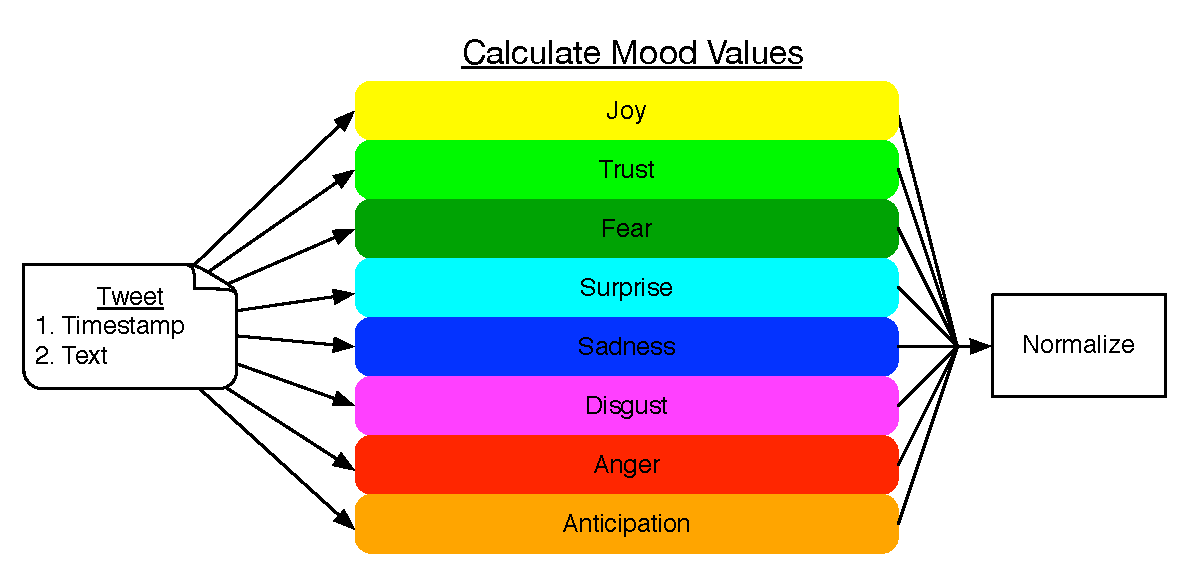
\includegraphics[width=0.53\textwidth]{sentiment_scoring.pdf}
\end{figure}
\end{center}
%\caption{\label{fig:frog1}Plutchik's wheel of emotion.}
%\end{wrapfigure}



%\spar The method for determining a tweets mood values is to do a word by word comparison of the words in the tweet to a set of words associated with each mood. If a word in the tweet exists in the list for a given mood, the value of that mood for that tweet is increased. Once every word in the tweet is processed, the values for the moods are normalized. 

\vspace{1em}
For example the tweet \emph{"I love to eat cake but I fear I will be angry after and look disgusting"} has the following normalized mood score: \vspace{1em}
\begin{table}[ht!]
\begin{tabular}{|l|l|l|l|l|l|l|l|}
\hline
\textbf{Joy} & \textbf{Trust} & \textbf{Fear} & \textbf{Surprise} & \textbf{Sadness} & \textit{\textbf{Disgust}} & \textit{\textbf{Anger}}  & \textbf{Anticipation} \\ \hline
0.0          & 0.2            & 0.2           & 0.0               & 0.2              & \multicolumn{1}{c|}{0.2}  & \multicolumn{1}{c|}{0.2} &          0.0             \\ \hline
\end{tabular}
\end{table}






\vspace{2em}

To handle the large amount of data, the sentiment analysis is implemented in the Map-Reduce framework Spark. Two months of data already results in approximately 88 million tweets. To process this size of data, we use Spark to calculate the sentiment of the tweets in a scalable fashion. The tweets are streamed into the application for both historical data as well as in periodic batches from the live stream.
    
    
\end{block}
\end{column}
\begin{column}{\twocolwid} % The second column

\begin{block}{Prediction of Stock Prices}

We attempt to correlate the daily mood with the closing price of the NASDAQ. The sentiment results from the day are analyzed using a feed forward neural network. Stock prices are aggregated with the average twitter mood data for each day, and this data is used to train the neural network. This algorithm has an average of 4.6\% error in it's prediction with a maximum error of 9.2\%. In the table below are the results of the last 7 days of the test data.

\begin{table}[ht!]
\begin{tabular}{|l|l|l|}
\hline
\textbf{Actual Stock Price} & \textbf{Predicted Stock Price} & \textbf{Percent Difference} \\ \hline
42.09                       & 42.45                          & 0.008                       \\ \hline
40.93                       & 42.25                          & 0.031                       \\ \hline
40.93                       & 42.23                          & 0.030                       \\ \hline
40.93                       & 42.51                          & 0.037                       \\ \hline
38.65                       & 42.60                          & 0.092                       \\ \hline
39.05                       & 42.24                          & 0.075                       \\ \hline
39.88                       & 42.00                          & 0.050                       \\ \hline
\end{tabular}
\end{table}


%\begin{figure}
%\begin{subfigure}[b]{0.2\textwidth}
%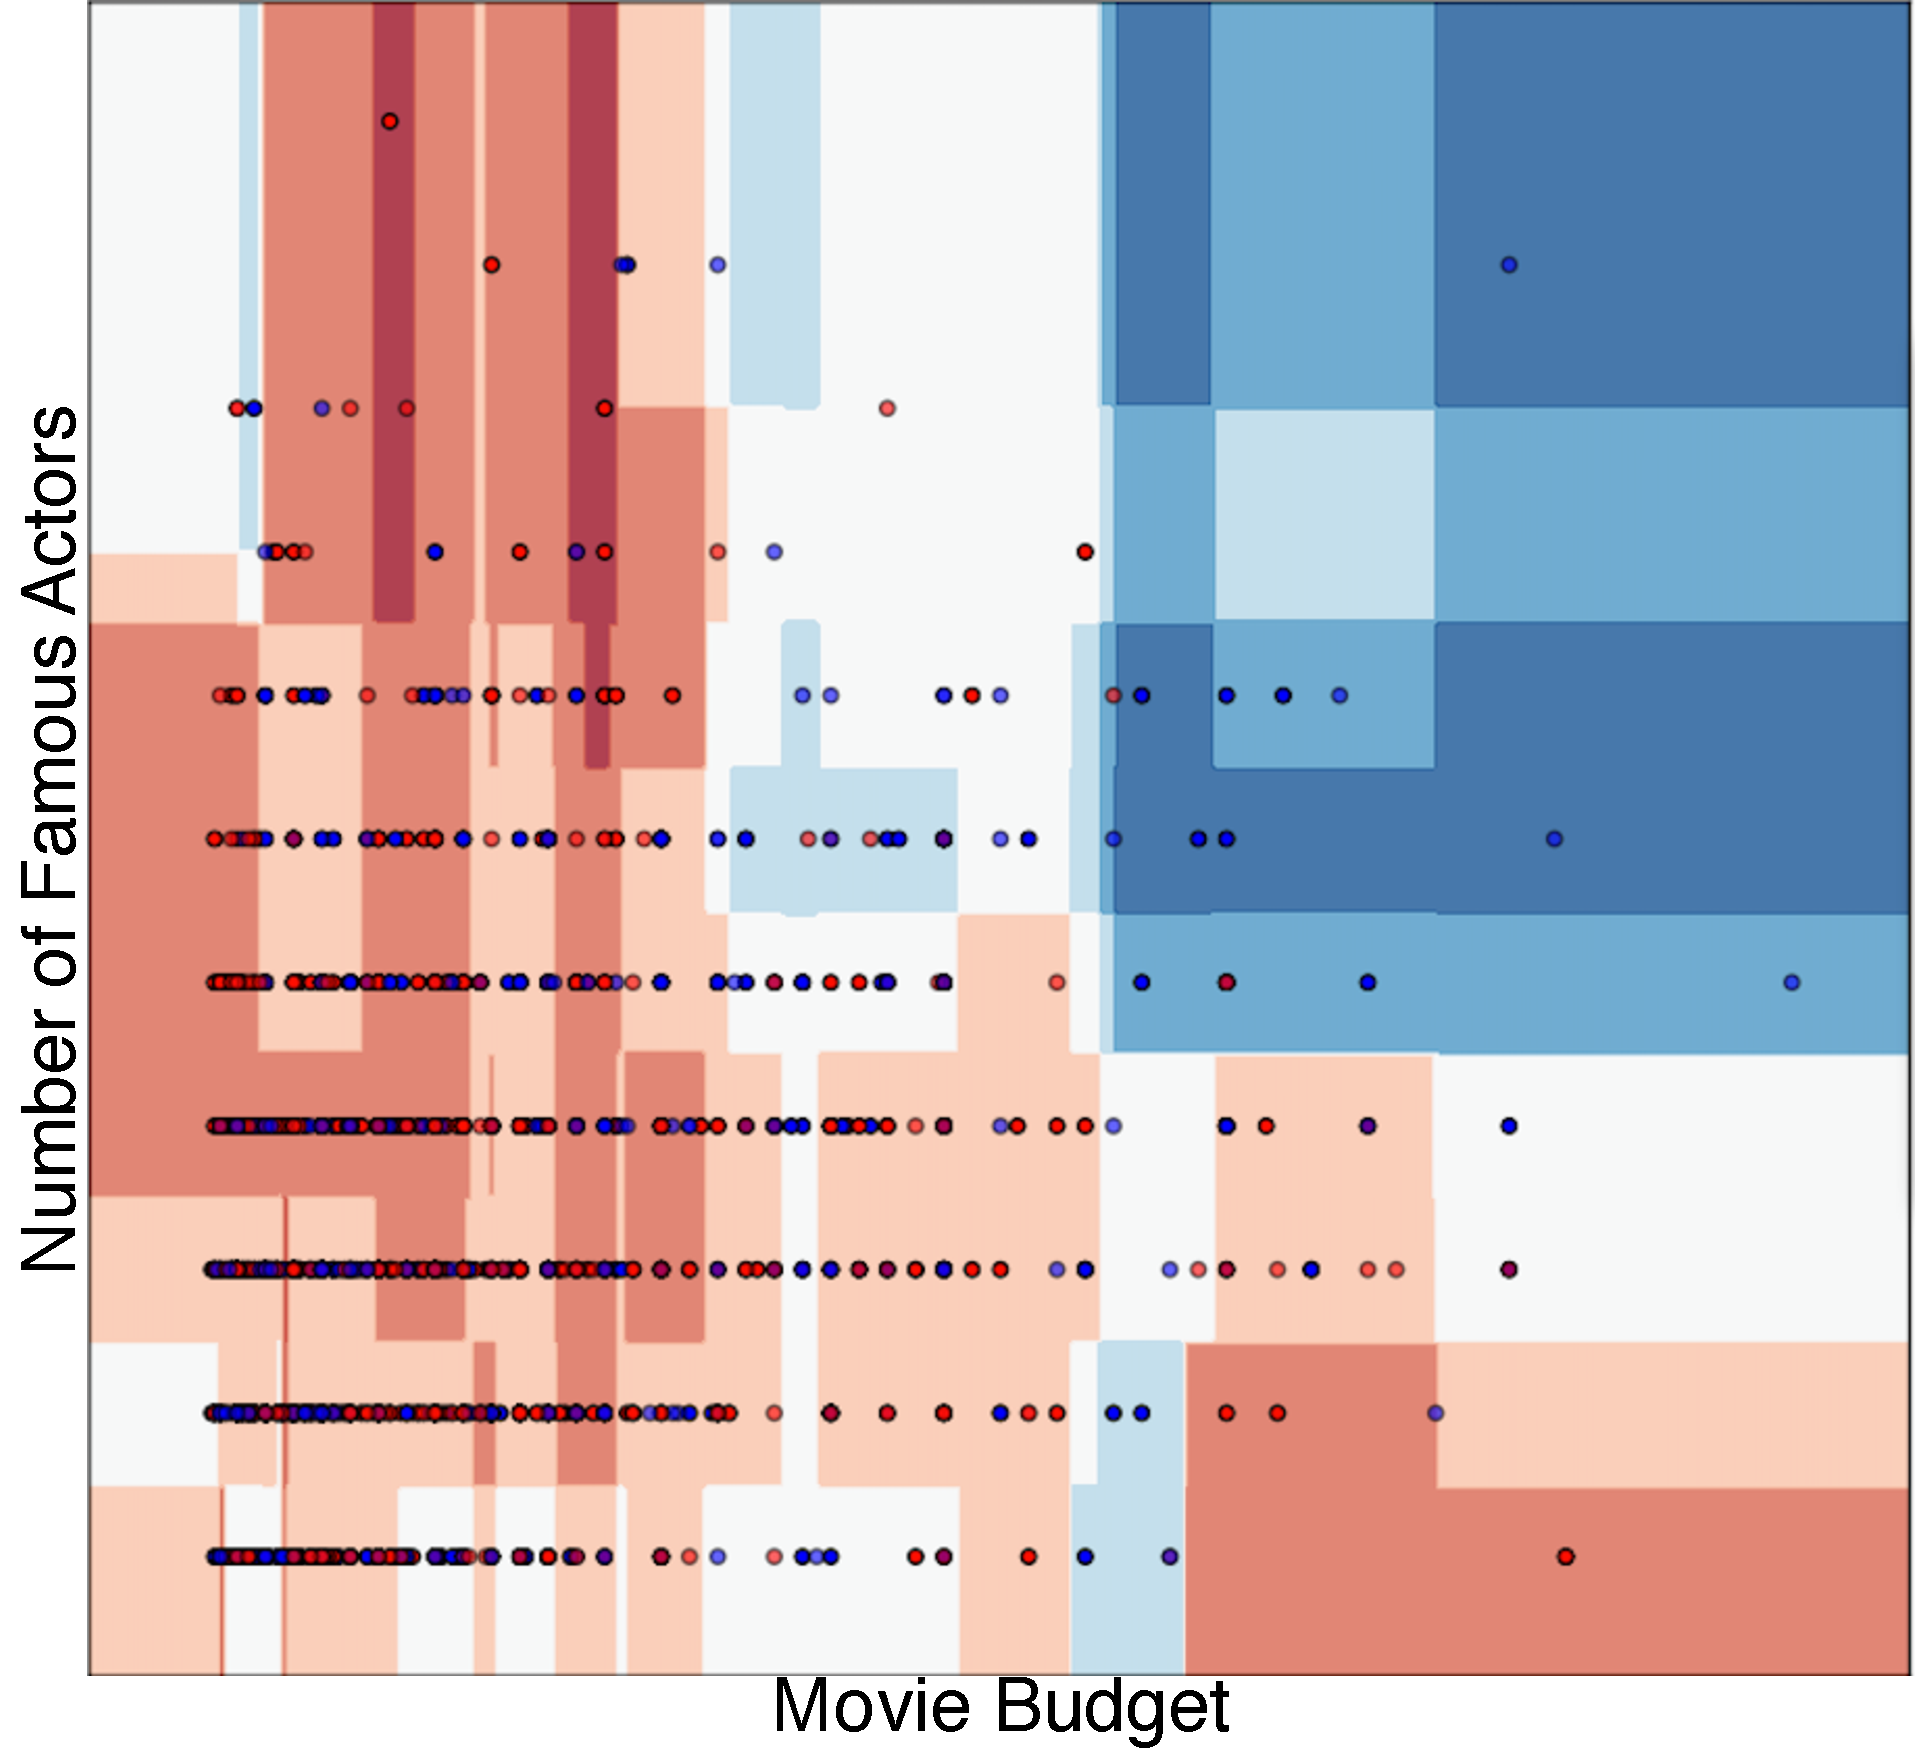
\includegraphics[width=30ex]{gb2.pdf}
%\caption{Gradient Boosting}
%\end{subfigure} \hspace{20ex}
%\begin{subfigure}[b]{0.2\textwidth}
% 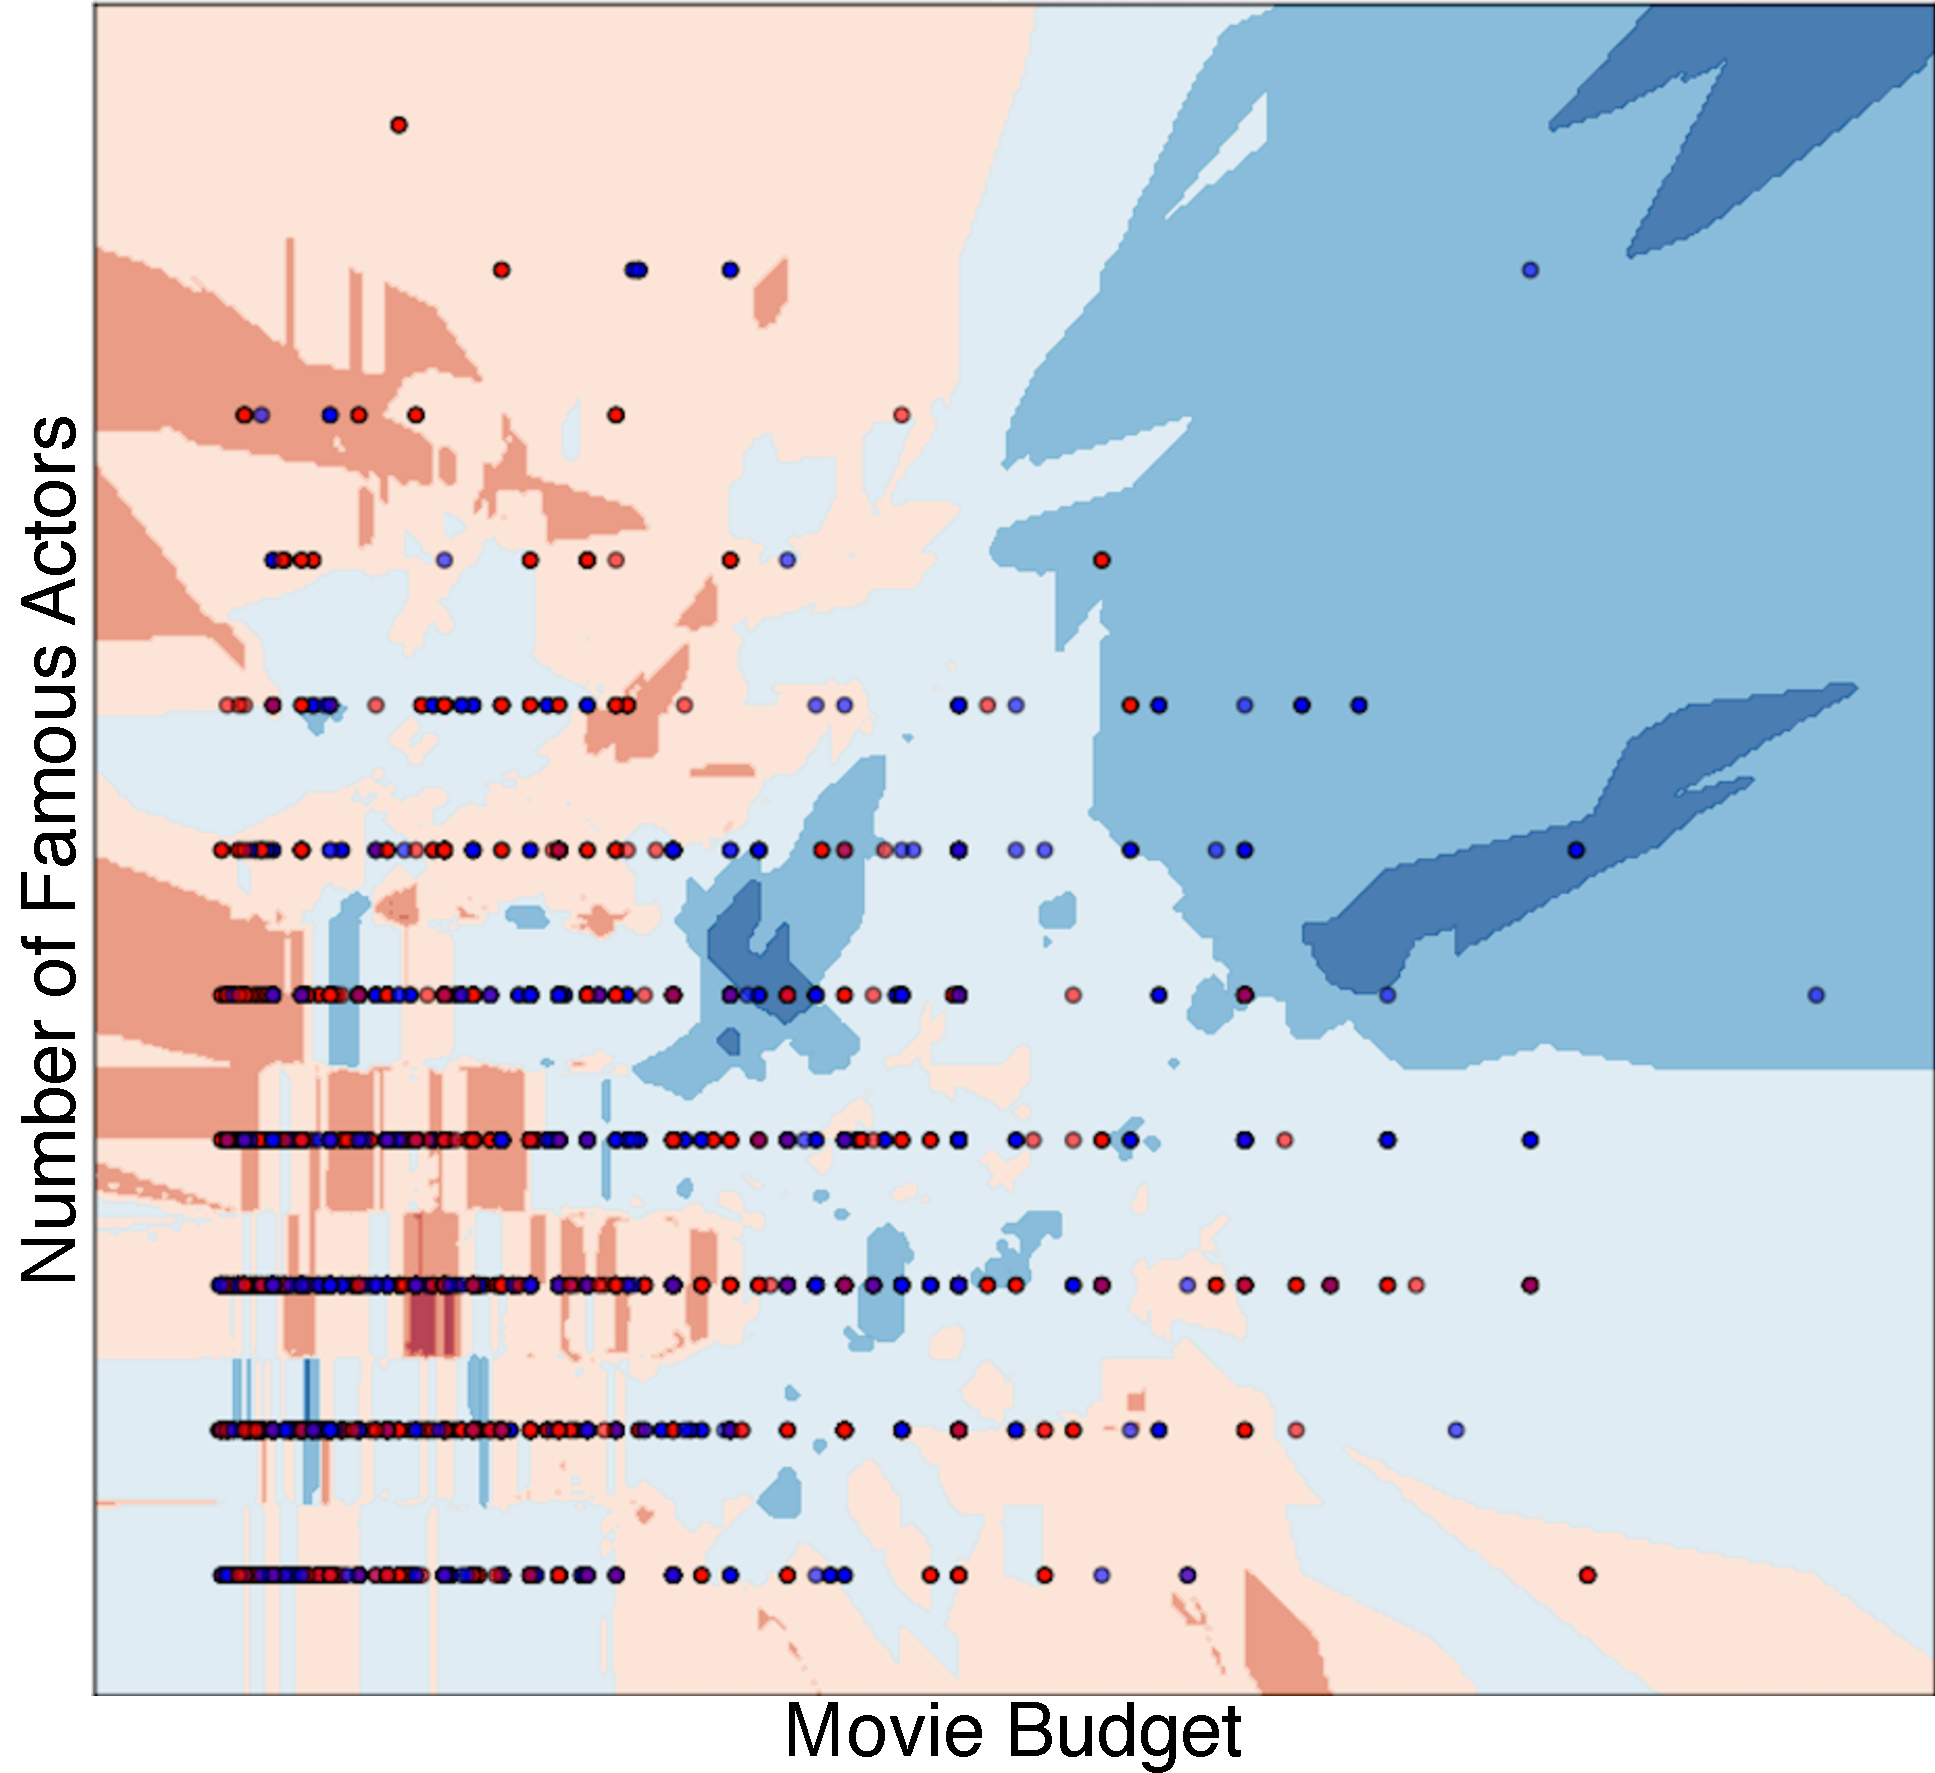
\includegraphics[width=30ex]{kn2.pdf}
 %\caption{KNeighbors, K=15}
 %\end{subfigure}
 %\caption{Classification of movies, Blue is success}
%\end{figure} 
\end{block}
\begin{block}{Interface}
Our tweets are gathered  from historical data or from the Twitter live stream and stored into a MongoDB.  The Map-Reduce framework Spark is used to process the tweets for the sentiment analysis. Finally, the \emph{ffnet} library in Python was used to build a neural network which we fed the sentiment data from the tweets to.
\begin{center}
\begin{figure}
	%\begin{subfigure}[b]{0.2\textwidth}
          %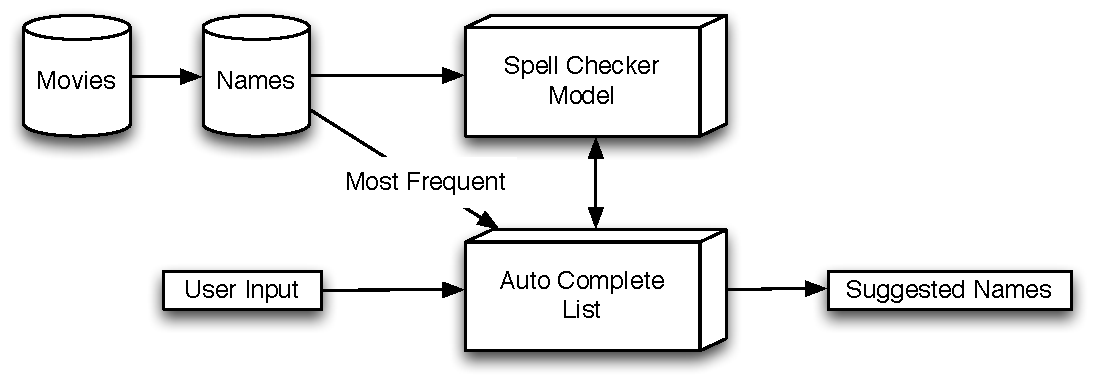
\includegraphics[width=40ex]{nameFig.pdf}
          %\caption{Autocomplete and autocorrect procedure}
         % \end{subfigure}\hspace{30ex}
          \includegraphics[width=60ex]{sitefinished.png}
          \caption{Website with most recent stock, mood, and prediction data.}
\end{figure}
\end{center}

\end{block}

\begin{block}{Conclusions}
\emph{We have performed an analysis on a large social network. We implemented a scalable system to perform sentiment analysis, which the results are used to create a prediction system for future stock prices. A prediction of future stock prices is done using a neural network. Finally, the results are updated in the interface on a continual basis. While we have implemented all the requirements for running the Twitter analysis and stock predictor, we so far are unable to discover a satisfactory correlation between moods and stock prices. }
\end{block}


\end{column}
\end{columns} % End of all the columns in the poster
\end{frame} % End of the enclosing frame
\end{document}